\documentclass{ximera}

%\usepackage{todonotes}

\newcommand{\todo}{}

\usepackage{esint} % for \oiint
\ifxake%%https://math.meta.stackexchange.com/questions/9973/how-do-you-render-a-closed-surface-double-integral
\renewcommand{\oiint}{{\large\bigcirc}\kern-1.56em\iint}
\fi


\graphicspath{
  {./}
  {ximeraTutorial/}
  {basicPhilosophy/}
  {functionsOfSeveralVariables/}
  {normalVectors/}
  {lagrangeMultipliers/}
  {vectorFields/}
  {greensTheorem/}
  {shapeOfThingsToCome/}
  {dotProducts/}
  {partialDerivativesAndTheGradientVector/}
  {../productAndQuotientRules/exercises/}
  {../normalVectors/exercisesParametricPlots/}
  {../continuityOfFunctionsOfSeveralVariables/exercises/}
  {../partialDerivativesAndTheGradientVector/exercises/}
  {../directionalDerivativeAndChainRule/exercises/}
  {../commonCoordinates/exercisesCylindricalCoordinates/}
  {../commonCoordinates/exercisesSphericalCoordinates/}
  {../greensTheorem/exercisesCurlAndLineIntegrals/}
  {../greensTheorem/exercisesDivergenceAndLineIntegrals/}
  {../shapeOfThingsToCome/exercisesDivergenceTheorem/}
  {../greensTheorem/}
  {../shapeOfThingsToCome/}
  {../separableDifferentialEquations/exercises/}
  {vectorFields/}
}

\newcommand{\mooculus}{\textsf{\textbf{MOOC}\textnormal{\textsf{ULUS}}}}

\usepackage{tkz-euclide}
\usepackage{tikz}
\usepackage{tikz-cd}
\usetikzlibrary{arrows}
\tikzset{>=stealth,commutative diagrams/.cd,
  arrow style=tikz,diagrams={>=stealth}} %% cool arrow head
\tikzset{shorten <>/.style={ shorten >=#1, shorten <=#1 } } %% allows shorter vectors

\usetikzlibrary{backgrounds} %% for boxes around graphs
\usetikzlibrary{shapes,positioning}  %% Clouds and stars
\usetikzlibrary{matrix} %% for matrix
\usepgfplotslibrary{polar} %% for polar plots
\usepgfplotslibrary{fillbetween} %% to shade area between curves in TikZ
%\usetkzobj{all}
\usepackage[makeroom]{cancel} %% for strike outs
%\usepackage{mathtools} %% for pretty underbrace % Breaks Ximera
%\usepackage{multicol}
\usepackage{pgffor} %% required for integral for loops



%% http://tex.stackexchange.com/questions/66490/drawing-a-tikz-arc-specifying-the-center
%% Draws beach ball
\tikzset{pics/carc/.style args={#1:#2:#3}{code={\draw[pic actions] (#1:#3) arc(#1:#2:#3);}}}



\usepackage{array}
\setlength{\extrarowheight}{+.1cm}
\newdimen\digitwidth
\settowidth\digitwidth{9}
\def\divrule#1#2{
\noalign{\moveright#1\digitwidth
\vbox{\hrule width#2\digitwidth}}}




% \newcommand{\RR}{\mathbb R}
% \newcommand{\R}{\mathbb R}
% \newcommand{\N}{\mathbb N}
% \newcommand{\Z}{\mathbb Z}

\newcommand{\sagemath}{\textsf{SageMath}}


%\renewcommand{\d}{\,d\!}
%\renewcommand{\d}{\mathop{}\!d}
%\newcommand{\dd}[2][]{\frac{\d #1}{\d #2}}
%\newcommand{\pp}[2][]{\frac{\partial #1}{\partial #2}}
% \renewcommand{\l}{\ell}
%\newcommand{\ddx}{\frac{d}{\d x}}

% \newcommand{\zeroOverZero}{\ensuremath{\boldsymbol{\tfrac{0}{0}}}}
%\newcommand{\inftyOverInfty}{\ensuremath{\boldsymbol{\tfrac{\infty}{\infty}}}}
%\newcommand{\zeroOverInfty}{\ensuremath{\boldsymbol{\tfrac{0}{\infty}}}}
%\newcommand{\zeroTimesInfty}{\ensuremath{\small\boldsymbol{0\cdot \infty}}}
%\newcommand{\inftyMinusInfty}{\ensuremath{\small\boldsymbol{\infty - \infty}}}
%\newcommand{\oneToInfty}{\ensuremath{\boldsymbol{1^\infty}}}
%\newcommand{\zeroToZero}{\ensuremath{\boldsymbol{0^0}}}
%\newcommand{\inftyToZero}{\ensuremath{\boldsymbol{\infty^0}}}



% \newcommand{\numOverZero}{\ensuremath{\boldsymbol{\tfrac{\#}{0}}}}
% \newcommand{\dfn}{\textbf}
% \newcommand{\unit}{\,\mathrm}
% \newcommand{\unit}{\mathop{}\!\mathrm}
% \newcommand{\eval}[1]{\bigg[ #1 \bigg]}
% \newcommand{\seq}[1]{\left( #1 \right)}
% \renewcommand{\epsilon}{\varepsilon}
% \renewcommand{\phi}{\varphi}


% \renewcommand{\iff}{\Leftrightarrow}

% \DeclareMathOperator{\arccot}{arccot}
% \DeclareMathOperator{\arcsec}{arcsec}
% \DeclareMathOperator{\arccsc}{arccsc}
% \DeclareMathOperator{\si}{Si}
% \DeclareMathOperator{\scal}{scal}
% \DeclareMathOperator{\sign}{sign}


%% \newcommand{\tightoverset}[2]{% for arrow vec
%%   \mathop{#2}\limits^{\vbox to -.5ex{\kern-0.75ex\hbox{$#1$}\vss}}}
% \newcommand{\arrowvec}[1]{{\overset{\rightharpoonup}{#1}}}
% \renewcommand{\vec}[1]{\arrowvec{\mathbf{#1}}}
% \renewcommand{\vec}[1]{{\overset{\boldsymbol{\rightharpoonup}}{\mathbf{#1}}}}

% \newcommand{\point}[1]{\left(#1\right)} %this allows \vector{ to be changed to \vector{ with a quick find and replace
% \newcommand{\pt}[1]{\mathbf{#1}} %this allows \vec{ to be changed to \vec{ with a quick find and replace
% \newcommand{\Lim}[2]{\lim_{\point{#1} \to \point{#2}}} %Bart, I changed this to point since I want to use it.  It runs through both of the exercise and exerciseE files in limits section, which is why it was in each document to start with.

% \DeclareMathOperator{\proj}{\mathbf{proj}}
% \newcommand{\veci}{{\boldsymbol{\hat{\imath}}}}
% \newcommand{\vecj}{{\boldsymbol{\hat{\jmath}}}}
% \newcommand{\veck}{{\boldsymbol{\hat{k}}}}
% \newcommand{\vecl}{\vec{\boldsymbol{\l}}}
% \newcommand{\uvec}[1]{\mathbf{\hat{#1}}}
% \newcommand{\utan}{\mathbf{\hat{t}}}
% \newcommand{\unormal}{\mathbf{\hat{n}}}
% \newcommand{\ubinormal}{\mathbf{\hat{b}}}

% \newcommand{\dotp}{\bullet}
% \newcommand{\cross}{\boldsymbol\times}
% \newcommand{\grad}{\boldsymbol\nabla}
% \newcommand{\divergence}{\grad\dotp}
% \newcommand{\curl}{\grad\cross}
%\DeclareMathOperator{\divergence}{divergence}
%\DeclareMathOperator{\curl}[1]{\grad\cross #1}
% \newcommand{\lto}{\mathop{\longrightarrow\,}\limits}

% \renewcommand{\bar}{\overline}

\colorlet{textColor}{black}
\colorlet{background}{white}
\colorlet{penColor}{blue!50!black} % Color of a curve in a plot
\colorlet{penColor2}{red!50!black}% Color of a curve in a plot
\colorlet{penColor3}{red!50!blue} % Color of a curve in a plot
\colorlet{penColor4}{green!50!black} % Color of a curve in a plot
\colorlet{penColor5}{orange!80!black} % Color of a curve in a plot
\colorlet{penColor6}{yellow!70!black} % Color of a curve in a plot
\colorlet{fill1}{penColor!20} % Color of fill in a plot
\colorlet{fill2}{penColor2!20} % Color of fill in a plot
\colorlet{fillp}{fill1} % Color of positive area
\colorlet{filln}{penColor2!20} % Color of negative area
\colorlet{fill3}{penColor3!20} % Fill
\colorlet{fill4}{penColor4!20} % Fill
\colorlet{fill5}{penColor5!20} % Fill
\colorlet{gridColor}{gray!50} % Color of grid in a plot

\newcommand{\surfaceColor}{violet}
\newcommand{\surfaceColorTwo}{redyellow}
\newcommand{\sliceColor}{greenyellow}




\pgfmathdeclarefunction{gauss}{2}{% gives gaussian
  \pgfmathparse{1/(#2*sqrt(2*pi))*exp(-((x-#1)^2)/(2*#2^2))}%
}


%%%%%%%%%%%%%
%% Vectors
%%%%%%%%%%%%%

%% Simple horiz vectors
\renewcommand{\vector}[1]{\left\langle #1\right\rangle}


%% %% Complex Horiz Vectors with angle brackets
%% \makeatletter
%% \renewcommand{\vector}[2][ , ]{\left\langle%
%%   \def\nextitem{\def\nextitem{#1}}%
%%   \@for \el:=#2\do{\nextitem\el}\right\rangle%
%% }
%% \makeatother

%% %% Vertical Vectors
%% \def\vector#1{\begin{bmatrix}\vecListA#1,,\end{bmatrix}}
%% \def\vecListA#1,{\if,#1,\else #1\cr \expandafter \vecListA \fi}

%%%%%%%%%%%%%
%% End of vectors
%%%%%%%%%%%%%

%\newcommand{\fullwidth}{}
%\newcommand{\normalwidth}{}



%% makes a snazzy t-chart for evaluating functions
%\newenvironment{tchart}{\rowcolors{2}{}{background!90!textColor}\array}{\endarray}

%%This is to help with formatting on future title pages.
\newenvironment{sectionOutcomes}{}{}



%% Flowchart stuff
%\tikzstyle{startstop} = [rectangle, rounded corners, minimum width=3cm, minimum height=1cm,text centered, draw=black]
%\tikzstyle{question} = [rectangle, minimum width=3cm, minimum height=1cm, text centered, draw=black]
%\tikzstyle{decision} = [trapezium, trapezium left angle=70, trapezium right angle=110, minimum width=3cm, minimum height=1cm, text centered, draw=black]
%\tikzstyle{question} = [rectangle, rounded corners, minimum width=3cm, minimum height=1cm,text centered, draw=black]
%\tikzstyle{process} = [rectangle, minimum width=3cm, minimum height=1cm, text centered, draw=black]
%\tikzstyle{decision} = [trapezium, trapezium left angle=70, trapezium right angle=110, minimum width=3cm, minimum height=1cm, text centered, draw=black]


\title{Shifted Exponential}

\begin{document}

\begin{abstract}
shifted range
\end{abstract}
\maketitle




The formula template for the basic exponential function looks like




\[  a \, r^x   \, \text{ with } \,  a, r \in \mathbb{R} \, | \,  r > 0   \]


As we have seen before, the coefficient $a$ controls vertical stretching or compression. The sign of $a$ dictates the sign of our function values. $r$ dictates a growing or decaying function.


Shifted exponential functions shift the range by adding a constant. \\


\[  a \, r^x  + b \, \text{ with } \,  a, b, r \in \mathbb{R} \, | \,  r > 0   \]




These no longer have a constant percent growth rate.  However, their analysis is exactly the same as for exponential functions with one big difference in our conclusions. Shifted exponential functions may have zeros. \\











\begin{example}  Shifted Exponential Function



Analyze   $f(x) = \frac{1}{3} \, 2^{x+5} - 7$ \\


\begin{explanation}

For the basic exponential function graph, the horizontal axis is the horizontal asymptote.  Here, this has been moved down $7$.



The ``inside'', representing the domain, is $x+5$.  This equals $0$, when $x=-5$.  The exponent is positive for $x>-5$, since the base is $2 > 1$, this is the direction of unbounded growth.  Therefore, the other direction (left) is where the horizontal asymptote is in effect.  Since the coefficient, $\frac{1}{3} > 0$, the unbounded growth is positive.

At $x=-5$, we have our one anchor point for the graph.  The point is $\left(-5, \frac{1}{3} - 7 \right)$, which is $\frac{1}{3}$ above the horizontal asymptote, $y = -7$.


Graph of $y = f(x)$.

\begin{image}
\begin{tikzpicture}
  \begin{axis}[
            domain=-10:10, ymax=10, xmax=10, ymin=-10, xmin=-10,
            axis lines =center, xlabel=$x$, ylabel=$y$, 
            ytick={-10,-8,-6,-4,-2,2,4,6,8,10},
            xtick={-10,-8,-6,-4,-2,2,4,6,8,10},
            ticklabel style={font=\scriptsize},
            every axis y label/.style={at=(current axis.above origin),anchor=south},
            every axis x label/.style={at=(current axis.right of origin),anchor=west},
            axis on top
          ]

          \addplot [line width=1, gray, dashed,samples=200,domain=(-10:10),<->] {-7};
          
          \addplot [line width=2, penColor, smooth,samples=200,domain=(-10:-0.6),<->] {0.33 * 2^(x+5)-7};

          \addplot[color=penColor,fill=penColor,only marks,mark=*] coordinates{(-5,6.666)};

         


 

  \end{axis}
\end{tikzpicture}
\end{image}




Our graph agrees with our analysis.

\begin{itemize}
\item The natural or implied domain of $f$ is $\mathbb{R}$.
\item $f$ is always increasing.
\item $f$ has no maximums or minimums.
\item $\lim\limits_{x \to -\infty} f(x) = -7$
\item $\lim\limits_{x \to \infty} f(x) = \infty$
\end{itemize}




\end{explanation}

\end{example}





















\begin{example}  Shifted Exponential Function



Analyze   $B(t) = -2 \, \left( \frac{2}{3} \right)^{3-t} + 4$ \\


\begin{observation}


First, observe that $\frac{2}{3} < \answer{1}$.


Our base is less than $1$.  Therefore, as its exponent gets large and positive, we multiply by more $\frac{2}{3}$'s and the overall values get smaller.


Except, the variable, $t$, in the exponent is multiplied by $-1$.  Therefore, we need $t$ to get large and negative in order for the exponent to get large and positve.


\begin{itemize}
\item $\left( \frac{2}{3} \right)^{3-t}$ decays when $t$ becomes more negative.
\item $\left( \frac{2}{3} \right)^{3-t}$ grows when $t$ becomes more positive.
\end{itemize}





\end{observation}



\begin{explanation}




\begin{model}

The exponential stem of $B(t)$ is $\left( \frac{2}{3} \right)^{-t}$, which is a transformed version of the basic exponential function model $M(t) = \left( \frac{2}{3} \right)^{t}$.  



When $t < 0$, then $-t > 0$ and we get  $\left( \frac{2}{3} \right)^{-t} = \left( \frac{2}{3} \right)^{positive}$ and the stem is becoming smaller, approaching $0$.  





\[ \lim\limits_{t \to -\infty} \left( \frac{2}{3} \right)^{-t} = 0 \]



When $t > 0$, then $-t < 0$ and we get  $\left( \frac{2}{3} \right)^{-t} = \left( \frac{2}{3} \right)^{negative}$ and the stem is becoming larger.  



\[ \lim\limits_{t \to \infty} \left( \frac{2}{3} \right)^{-t} = \infty \]








\end{model}

Next, we have a negative leading coefficient. \\

Since $-2 < 0$, the values of $-2 \, \left( \frac{2}{3} \right)^{power}$ are always negative.



Finally, we also have two shifts:



$\blacktriangleright$ \textbf{\textcolor{blue!55!black}{Vertical Shift}} 

Adding $4$ to the outside shifts the graph vertically up $4$.  The asymptote is $y = 4$ and 

\[ \lim\limits_{t \to -\infty} B(t) = 4 \]




$\blacktriangleright$ \textbf{\textcolor{blue!55!black}{Horizontal Shift}} 

Our exponent is $3 - t = -t + 3$.  Our anchor point for graphing is associated with the exponent equalling $0$.



$3-t=0$ when $t=3$. Our one anchor point is shifted over to $3$.  Multipying by $-2$, means the dot is $2$ away from the horizontal asymptote, which is now $y=4$.










Graph of $y = B(t)$.

\begin{image}
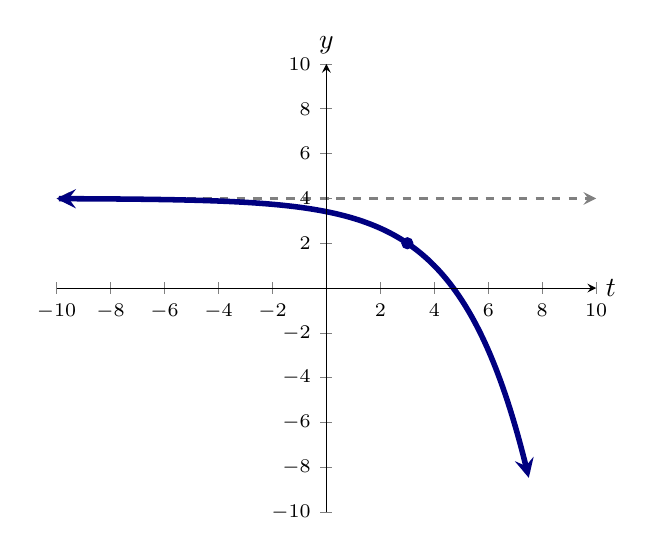
\begin{tikzpicture}
  \begin{axis}[
            domain=-10:10, ymax=10, xmax=10, ymin=-10, xmin=-10,
            axis lines =center, xlabel=$t$, ylabel=$y$, 
            ytick={-10,-8,-6,-4,-2,2,4,6,8,10},
            xtick={-10,-8,-6,-4,-2,2,4,6,8,10},
            ticklabel style={font=\scriptsize},
            every axis y label/.style={at=(current axis.above origin),anchor=south},
            every axis x label/.style={at=(current axis.right of origin),anchor=west},
            axis on top
          ]
          
          \addplot [line width=1, gray, dashed,samples=200,domain=(-10:10),<->] {4};

          \addplot [line width=2, penColor, smooth,samples=200,domain=(-10:7.5),<->] {-2 * (0.666^(3-x)) + 4};

          \addplot[color=penColor,fill=penColor,only marks,mark=*] coordinates{(3,2)};

          


  \end{axis}
\end{tikzpicture}
\end{image}




Our graphical analysis tells us that 

\begin{itemize}
\item The natural or implied domain of $B$ is $\mathbb{R}$.
\item $B$ is always decreasing.
\item $B$ has no maximums or minimums.
\item $\lim\limits_{t \to -\infty} B(t) = 4$
\item $\lim\limits_{t \to \infty} B(t) = -\infty$
\end{itemize}


\end{explanation}

\end{example}






















\begin{center}
\textbf{\textcolor{green!50!black}{ooooo=-=-=-=-=-=-=-=-=-=-=-=-=ooOoo=-=-=-=-=-=-=-=-=-=-=-=-=ooooo}} \\

more examples can be found by following this link\\ \link[More Examples of Percent Change]{https://ximera.osu.edu/csccmathematics/precalculus1/precalculus1/percentChange/examples/exampleList}

\end{center}





\end{document}
